% Created 2017-10-21 Sat 17:24
\documentclass[a4paper]{article}
\usepackage[utf8]{inputenc}
\usepackage[T1]{fontenc}
\usepackage{fixltx2e}
\usepackage{graphicx}
\usepackage{longtable}
\usepackage{float}
\usepackage{wrapfig}
\usepackage{rotating}
\usepackage[normalem]{ulem}
\usepackage{amsmath}
\usepackage{textcomp}
\usepackage{marvosym}
\usepackage{wasysym}
\usepackage{amssymb}
\usepackage{hyperref}
\tolerance=1000
\usepackage{minted}
\usepackage[margin=0.8in]{geometry}
\usepackage{amssymb,amsmath}
\usepackage{fancyhdr} %For headers and footers
\pagestyle{fancy} %For headers and footers
\usepackage{lastpage} %For getting page x of y
\usepackage{float} %Allows the figures to be positioned and formatted nicely
\restylefloat{figure} %and this command
\usepackage{hyperref}
\hypersetup{urlcolor=blue}
\usepackage{minted}
\setminted{frame=single,framesep=10pt}
\chead{}
\rhead{\today}
\cfoot{}
\rfoot{\thepage\ of \pageref{LastPage}}
\usepackage[parfill]{parskip}
\usepackage{subfig}
\hypersetup{colorlinks=true,linkcolor=black}
\usepackage{framed}
\author{Nathan Hughes (\href{mailto:nah31@aber.ac.uk}{nah26@aber.ac.uk})}
\date{\today}
\title{Assignment 1}
\hypersetup{
  pdfkeywords={},
  pdfsubject={},
  pdfcreator={Emacs 25.3.1 (Org mode 8.2.10)}}
\begin{document}

\maketitle
\vspace{2cm}

\begin{center}

\includegraphics[width=4cm]{./ruby.png}
\end{center}

\clearpage
\tableofcontents
\clearpage


\section{Introduction}
\label{sec-1}

\section{Steps taken}
\label{sec-2}

\subsection{Creating a new rails site}
\label{sec-2-1}
\begin{listing}[H]
\begin{minted}[]{bash}
rails new csa
\end{minted}
\caption{Editing File X}
\end{listing}

\subsection{Generating Scaffolds for Users and Posts}
\label{sec-2-2}
\begin{listing}[H]
\begin{minted}[]{bash}
rails g scaffold Post title
rails g scaffold Users surname forename phone grad_year:integer jobs:boolean email
\end{minted}
\caption{Editing File X}
\end{listing}

\subsection{Adding constraints to Users}
\label{sec-2-3}
\begin{listing}[H]
\begin{minted}[]{ruby}
class CreateUsers < ActiveRecord::Migration[5.1]
  def change
    create_table :users do |t|
      t.string :surname, null:false
      t.string :forename, null:false
      t.string :phone
      t.integer :grad_year, null:false
      t.boolean :jobs, default: false
      t.string :email, null:false

      t.timestamps
    end

    add_index:users,:surname
    add_index:users,:email

  end
end
\end{minted}
\caption{Editing File X}
\end{listing}

\subsection{Change index routing to Posts}
\label{sec-2-4}
\begin{listing}[H]
\begin{minted}[]{ruby}
Rails.application.routes.draw do
  resources :users
  resources :posts

  root 'posts#index'

end
\end{minted}
\caption{Editing File X}
\end{listing}

\subsection{Update these changes and migrate to the Database}
\label{sec-2-5}
\begin{listing}[H]
\begin{minted}[]{bash}
rails db:migrate
\end{minted}
\caption{Editing File X}
\end{listing}

\subsection{Adding Users and Body to Posts}
\label{sec-2-6}

\subsubsection{Creating a migrate file for adding body}
\label{sec-2-6-1}
\begin{listing}[H]
\begin{minted}[]{bash}
rails g migration add_body_to_posts body:text
\end{minted}
\caption{Editing File X}
\end{listing}

\subsubsection{Creating a migrate file for linking tables}
\label{sec-2-6-2}
\begin{listing}[H]
\begin{minted}[]{bash}
rails g migration add_user_to_posts user:references
\end{minted}
\caption{Editing File X}
\end{listing}

\subsubsection{Update Post model}
\label{sec-2-6-3}
\begin{listing}[H]
\begin{minted}[]{ruby}
class Post < ApplicationRecord
  validates_presence_of :title

  belongs_to :user,optional: true
end
\end{minted}
\caption{Editing File X}
\end{listing}
\subsubsection{Update User model}
\label{sec-2-6-4}
\begin{listing}[H]
\begin{minted}[]{ruby}
class User < ApplicationRecord
  has_many :posts,
	   dependent: :destroy
end
\end{minted}
\caption{Editing File X}
\end{listing}


\subsubsection{Updating views for Posts form}
\label{sec-2-6-5}
To do this we edit the view component of posts, which was generated by the initial scaffold commands
\begin{listing}[H]
\begin{minted}[]{bash}
<div class="field">
  <%= form.label :email %>
  <%= if post.user
    text_field_tag 'email',post.user.email
  else
    text_field_tag 'email'
  end %>
</div>

<div class="field">
  <%= form.label :body %><br>
  <%= form.text_area :body %>
</div>
\end{minted}
\caption{Editing File X}
\end{listing}

\subsubsection{Updating view for Posts listing}
\label{sec-2-6-6}
\begin{listing}[H]
\begin{minted}[]{bash}
<p>
  <strong>Title:</strong>
  <%= @post.title %>
</p>

<p>
  <strong>Email:</strong>
  <% if @post.user %>
    <%= link_to "#{@post.user.email}", @post.user %>
  <% else %>
    Anonymous
  <% end %>
</p>

<p>
  <%= @post.body %>
</p>
\end{minted}
\caption{Editing File X}
\end{listing}



\subsection{{\bfseries\sffamily TODO} Paginations}
\label{sec-2-7}

\subsection{{\bfseries\sffamily TODO} Tabbing}
\label{sec-2-8}

\section{{\bfseries\sffamily TODO} MVC Model}
\label{sec-3}

\subsection{{\bfseries\sffamily TODO} UML Diagram}
\label{sec-3-1}


\subsubsection{Database}
\label{sec-3-1-1}
\begin{center}
\begin{figure}[htb]
\centering
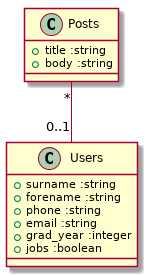
\includegraphics[width=4cm]{posts-users.png}
\caption{Posts and Users UML}
\end{figure}
\end{center}

\subsubsection{{\bfseries\sffamily TODO} What is the Model-2 Variant}
\label{sec-3-1-2}
\subsection{{\bfseries\sffamily TODO} Models}
\label{sec-3-2}
\subsection{{\bfseries\sffamily TODO} Views}
\label{sec-3-3}
\subsection{{\bfseries\sffamily TODO} Controls}
\label{sec-3-4}


\section{Database}
\label{sec-4}

\subsection{{\bfseries\sffamily TODO} Database location}
\label{sec-4-1}

\subsection{{\bfseries\sffamily TODO} Migration Files}
\label{sec-4-2}
\begin{minted}[]{bash}
rails db:migrate
\end{minted}
% Emacs 25.3.1 (Org mode 8.2.10)
\end{document}